\subsection{Clasificación de imágenes para localización}

Una aplicación de uno de los servicios que brinda la API REST
y que además fue desarrollado por el LAR es la clasificación de
imágenes en cuatro clases, donde cada clase representa
un escenario dentro dentro del área del laboratorio. Este servicio de procesamiento de imágenes permite que el robot conozca en qué espacio se encuentra al navegar en esta zona.

\subsubsection{Objetivos}

\begin{itemize}
    \item Implementar un modelo de aprendizaje profundo.
    \item Consumir el modelo de aprendizaje profundo como un servicio web.
\end{itemize}

\subsubsection{Problema}


El problema de clasificación de imágenes es la tarea de asignarle a una imagen de
entrada una etiqueta a partir de un conjunto de categorías. Este es uno de los principales
problemas dentro del campo de la visión computacional, que a pesar de su simplicidad
tiene bastantes aplicaciones prácticas. Entre esas aplicaciones, muchas interesan al
campo de la robótica móvil, por ejemplo, para la navegación de un robot de manera
autónoma, nos gustaría que supiera en que lugar está simplemente con una fotografía
que obtenga en ese momento desde sus cámaras, así podría saber si ha llegado al 
lugar de su objetivo, o a partir de la zona donde se ubica planear una trayectoria.

\subsubsection{Solución}


Se implementó en TensorFlow un modelo para clasificar imágenes
de algunos lugares sobre los que podría navegar el robot Fibonacho. 

El modelo es
una red neuronal convolucional, que recibe como entrada un arreglo con los
pixeles de una imagen tomada por el robot, y la salida es la categoría a la que pertenece esa imagen. 
Las clases en las que se desea clasificar las imágenes son lugares alrededor
del Laboratorio de Algoritmos para la Robótica, que se ubica en el cubículo $15$ del
Centro de Desarrollo Tecnológico de la FES Acatlán. Se eligieron las siguientes cuatro zonas:

\begin{itemize}
    \item El cubículo.
    \item La salida de emergencia.
    \item La cancha de entrenamiento de fútbol para el robot NAO.
    \item Zona de trabajo del Laboratorio.
\end{itemize}

Los modelos elaborados en TensorFlow contienen la gráfica de cómputo
y los valores de los parámetros que se han entrenado. Estos datos
están contenidos en varios archivos que se pueden guardar para
entrenamientos posteriores o para realizar inferencias sobre 
un modelo cuyas variables han sido aprendidas.


La API REST se encarga de restaurar la gráfica y valores del modelo para que al recibir una imagen enviada por el robot
Fibonacho  o cualquier otro
dispositivo cliente se envíe en el cuerpo de la respuesta
un JSON con la cadena que identifica a la categoría 
inferida.

\subsubsection{Resultados}

Se hicieron $40$ solicitudes a la API REST desde el robot,
$10$ por cada categoría. Esto es, se enviaron
$10$ imágenes de la cancha, $10$ de la salida,
$10$ del cubículo y $10$ del área de trabajo.
En las tablas \ref{table:soccer_nao_results},
\ref{table:exit}, \ref{table:desks} y
\ref{table:office}, se resumen los resultados obtenidos.
En la figura \ref{nao_api_images} se muestran algunas imágenes capturadas en las pruebas.


Se puede ver que existen más aciertos
con imágenes de la cancha de fútbol, 8 de 10 inferencias correctas.
Clasificando imágenes de la salida de emergencia
y del cubículo se tienen 7 de 10 predicciones correctas.
Para el área de trabajo tuvo su peor desempeño con 6 de
10 aciertos. Si bien no se obtiene
la precisión reportada durante el
entrenamiento del modelo, el tiempo
de ejecución y los
resultados son buenos
para la funcionalidad de
auxiliar a la navegación del robot.
El tiempo de solicitud y repuesta varía entre peticiones.
Factores que influyen al tiempo son el tamaño de la 
imagen enviada y la velocidad de la conexión del cliente
y del servidor. 

\begin{table}[!h]
\centering
\begin{tabular}{|l|l|l|l|}
\hline
Clase        & Predicción   & Tiempo        & Correcta \\ \hline
cancha & z. trabajo        & 3.0337650776 & F        \\ \hline
cancha & cancha & 3.0559039116 & T        \\ \hline
cancha & z. trabajo        & 2.09687018394 & F        \\ \hline
cancha & cancha & 3.0169699192 & T        \\ \hline
cancha & z. trabajo        & 2.32713413239 & F        \\ \hline
cancha & cancha & 3.0284428596 & T        \\ \hline
cancha & cancha & 3.0252449512 & T        \\ \hline
cancha & cancha & 3.1204240322 & T        \\ \hline
cancha & cancha & 3.013076067  & T        \\ \hline
cancha & cancha & 3.2163701057 & T        \\ \hline
\end{tabular}
\caption{Resultados de las imágenes de la cancha de fútbol.}
\label{table:soccer_nao_results}
\end{table}

\begin{table}[!h]
\centering
\begin{tabular}{|l|l|l|l|}
\hline
Clase & Predicción & Tiempo        & Correcta \\ \hline
salida  & salida       & 3.2262349129 & T     \\ \hline
salida  & salida       & 3.0402858257 & T     \\ \hline
salida  & salida     & 3.298979044  & T    \\ \hline
salida  & cubículo     & 3.6488580704 & F    \\ \hline
salida  & salida       & 3.4767799377 & T     \\ \hline
salida  & salida       & 3.6147930622 & T     \\ \hline
salida  & salida       & 3.7430388927 & T     \\ \hline
salida  & cubículo     & 3.7496609688 & F    \\ \hline
salida  & salida       & 3.8713350296 & T     \\ \hline
salida  & cubículo     & 4.0420210361 & F    \\ \hline
\end{tabular}
\caption{Resultados para fotografías de la salida de emergencia.}
\label{table:exit}
\end{table}

\begin{table}[!h]
\centering
\begin{tabular}{|l|l|l|l|}
\hline
Clase      & Predicción & Tiempo        & Correcta \\ \hline
z. trabajo & z. trabajo & 5.3504459858 & T        \\ \hline
z. trabajo & cubículo    & 5.2893049717 & F        \\ \hline
z. trabajo & cubículo    & 5.2149860859 & F        \\ \hline
z. trabajo & z. trabajo & 5.2179970741 & T        \\ \hline
z. trabajo & cubículo    & 5.6882929802 & F        \\ \hline
z. trabajo & cubículo    & 5.6848390102 & F        \\ \hline
z. trabajo & z. trabajo & 5.9792921543 & T        \\ \hline
z. trabajo & z. trabajo & 5.8859920502 & T        \\ \hline
z. trabajo & z. trabajo & 5.722206831  & T        \\ \hline
z. trabajo & z. trabajo & 6.7581658363 & T        \\ \hline
\end{tabular}
\caption{Resultados para la fotografías del área
de trabajo.}
\label{table:desks}
\end{table}

\begin{table}[!h]
\centering
\begin{tabular}{|l|l|l|l|}
\hline
Clase   & Predicción & Tiempo        & Correcta \\ \hline
cubículo & cubículo    & 3.5342819691 & T        \\ \hline
cubículo & cubículo    & 3.9999611378 & T        \\ \hline
cubículo & z. trabajo & 4.6536300182 & F        \\ \hline
cubículo & z. trabajo & 3.8637499809 & F        \\ \hline
cubículo & z. trabajo & 4.887745142  & F        \\ \hline
cubículo & cubículo    & 4.4888358116 & T        \\ \hline
cubículo & cubículo    & 4.6198430061 & T        \\ \hline
cubículo & cubículo    & 4.4448840618 & T        \\ \hline
cubículo & cubículo    & 4.5735599995 & T        \\ \hline
cubículo & cubículo    & 5.2998209    & T        \\ \hline
\end{tabular}
\caption{Resultados de obtenidos con imágenes del cubículo.}
\label{table:office}
\end{table}

\begin{figure}[!ht] 
  \centering
\subfloat[Clase = cancha, predicción = cancha. Tiempo = 3.05]{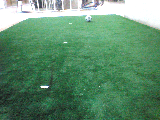
\includegraphics[scale=1]{nao_api_soccer}}
\qquad
\subfloat[Clase = salida, predicción = salida. Tiempo = 3.29]{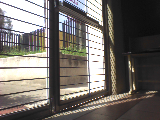
\includegraphics[scale=1]{exit_incorrect}}
\qquad
\subfloat[Clase = zona de trabajo, predicción = cubículo. Tiempo = 5.21]{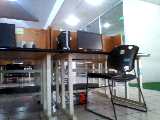
\includegraphics[scale=1]{deks_incorrect}}
\qquad
\subfloat[Clase = cubículo, predicción = cubículo. Tiempo = 3.53]{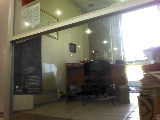
\includegraphics[scale=1]{nao_api_office}}
\caption{Predicciones hechas enviando imágenes del robot a la API REST. El tiempo son los
segundos que se tardó en enviar la solicitud y en recibir la respuesa. \label{nao_api_images}}
\end{figure}
